\documentclass[tikz,border=3.14mm]{standalone}
\usepackage{pgfplots}
\pgfplotsset{compat=1.17}

\begin{document}

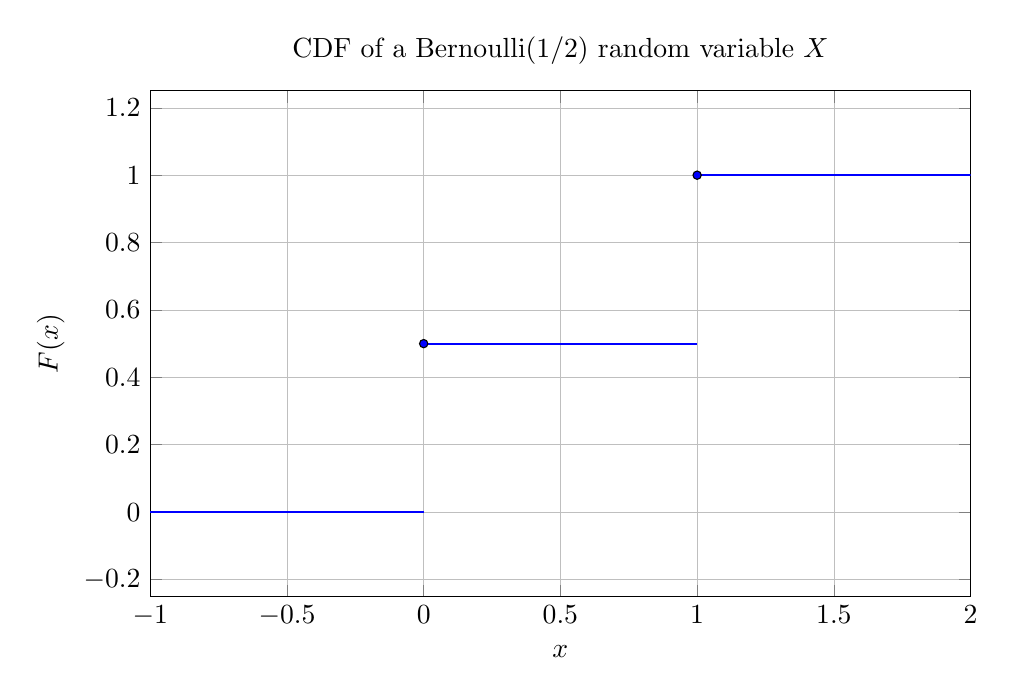
\begin{tikzpicture}
    \begin{axis}[
        xlabel = \(x\),
        ylabel = {$F(x)$},
        domain = -.4:4,
        xmax = 2,
        xmin = -1,
        ymin = -0.25,
        ymax = 1.25,
        samples = 100,
        title = {CDF of a Bernoulli(1/2) random variable $X$},
        width = 12cm,
        height = 8cm,
    grid=both,
    grid style={line width=.1pt, draw=gray!10},
    major grid style={line width=.2pt,draw=gray!50},
    ]
    
    \addplot[blue, thick, no markers] (-1,0) -- (0,0);
    \addplot[blue, thick, no markers] (0,.5) -- (1,.5);
    \addplot[blue, thick, no markers] (1,1) -- (2,1);

    \node [circle, inner sep = 0mm, draw, fill = blue, minimum size = 3pt] at (0,.5) {};
    \node [circle, inner sep = 0mm, draw, fill = blue, minimum size = 3pt] at (1,1) {};
    
    \end{axis}
\end{tikzpicture}

\end{document}
